\documentclass[11pt]{article}
% NOTE: Add in the relevant information to the commands below; or, if you'll be using the same information frequently, add these commands at the top of paolo-pset.tex file. 
\newcommand{\name}{Agustín Esteva}
\newcommand{\email}{aesteva@uchicago.edu}
\newcommand{\classnum}{207}
\newcommand{\subject}{Honors Analysis in $\bbR^n$}
\newcommand{\instructors}{Luis Silvestre}
\newcommand{\assignment}{Problem Set 4}
\newcommand{\semester}{Fall 2024}
\newcommand{\duedate}{2024-28-10}
\newcommand{\bA}{\mathbf{A}}
\newcommand{\bB}{\mathbf{B}}
\newcommand{\bC}{\mathbf{C}}
\newcommand{\bD}{\mathbf{D}}
\newcommand{\bE}{\mathbf{E}}
\newcommand{\bF}{\mathbf{F}}
\newcommand{\bG}{\mathbf{G}}
\newcommand{\bH}{\mathbf{H}}
\newcommand{\bI}{\mathbf{I}}
\newcommand{\bJ}{\mathbf{J}}
\newcommand{\bK}{\mathbf{K}}
\newcommand{\bL}{\mathbf{L}}
\newcommand{\bM}{\mathbf{M}}
\newcommand{\bN}{\mathbf{N}}
\newcommand{\bO}{\mathbf{O}}
\newcommand{\bP}{\mathbf{P}}
\newcommand{\bQ}{\mathbf{Q}}
\newcommand{\bR}{\mathbf{R}}
\newcommand{\bS}{\mathbf{S}}
\newcommand{\bT}{\mathbf{T}}
\newcommand{\bU}{\mathbf{U}}
\newcommand{\bV}{\mathbf{V}}
\newcommand{\bW}{\mathbf{W}}
\newcommand{\bX}{\mathbf{X}}
\newcommand{\bY}{\mathbf{Y}}
\newcommand{\bZ}{\mathbf{Z}}

%% blackboard bold math capitals
\newcommand{\bbA}{\mathbb{A}}
\newcommand{\bbB}{\mathbb{B}}
\newcommand{\bbC}{\mathbb{C}}
\newcommand{\bbD}{\mathbb{D}}
\newcommand{\bbE}{\mathbb{E}}
\newcommand{\bbF}{\mathbb{F}}
\newcommand{\bbG}{\mathbb{G}}
\newcommand{\bbH}{\mathbb{H}}
\newcommand{\bbI}{\mathbb{I}}
\newcommand{\bbJ}{\mathbb{J}}
\newcommand{\bbK}{\mathbb{K}}
\newcommand{\bbL}{\mathbb{L}}
\newcommand{\bbM}{\mathbb{M}}
\newcommand{\bbN}{\mathbb{N}}
\newcommand{\bbO}{\mathbb{O}}
\newcommand{\bbP}{\mathbb{P}}
\newcommand{\bbQ}{\mathbb{Q}}
\newcommand{\bbR}{\mathbb{R}}
\newcommand{\bbS}{\mathbb{S}}
\newcommand{\bbT}{\mathbb{T}}
\newcommand{\bbU}{\mathbb{U}}
\newcommand{\bbV}{\mathbb{V}}
\newcommand{\bbW}{\mathbb{W}}
\newcommand{\bbX}{\mathbb{X}}
\newcommand{\bbY}{\mathbb{Y}}
\newcommand{\bbZ}{\mathbb{Z}}

%% script math capitals
\newcommand{\sA}{\mathscr{A}}
\newcommand{\sB}{\mathscr{B}}
\newcommand{\sC}{\mathscr{C}}
\newcommand{\sD}{\mathscr{D}}
\newcommand{\sE}{\mathscr{E}}
\newcommand{\sF}{\mathscr{F}}
\newcommand{\sG}{\mathscr{G}}
\newcommand{\sH}{\mathscr{H}}
\newcommand{\sI}{\mathscr{I}}
\newcommand{\sJ}{\mathscr{J}}
\newcommand{\sK}{\mathscr{K}}
\newcommand{\sL}{\mathscr{L}}
\newcommand{\sM}{\mathscr{M}}
\newcommand{\sN}{\mathscr{N}}
\newcommand{\sO}{\mathscr{O}}
\newcommand{\sP}{\mathscr{P}}
\newcommand{\sQ}{\mathscr{Q}}
\newcommand{\sR}{\mathscr{R}}
\newcommand{\sS}{\mathscr{S}}
\newcommand{\sT}{\mathscr{T}}
\newcommand{\sU}{\mathscr{U}}
\newcommand{\sV}{\mathscr{V}}
\newcommand{\sW}{\mathscr{W}}
\newcommand{\sX}{\mathscr{X}}
\newcommand{\sY}{\mathscr{Y}}
\newcommand{\sZ}{\mathscr{Z}}


\renewcommand{\emptyset}{\O}

\newcommand{\abs}[1]{\lvert #1 \rvert}
\newcommand{\norm}[1]{\lVert #1 \rVert}
\newcommand{\sm}{\setminus}



\newcommand{\sarr}{\rightarrow}
\newcommand{\arr}{\longrightarrow}

% NOTE: Defining collaborators is optional; to not list collaborators, comment out the line below.
%\newcommand{\collaborators}{Alyssa P. Hacker (\texttt{aphacker}), Ben Bitdiddle (\texttt{bitdiddle})}

\input{paolo-pset.tex}

% NOTE: To compile a version of this pset without problems, solutions, or reflections, uncomment the relevant line below.

%\excludeversion{problem}
%\excludeversion{solution}
%\excludeversion{reflection}

\begin{document}	
	
	% Use the \psetheader command at the beginning of a pset. 
	\psetheader

\section*{Problem 1}
\begin{problem}
Let $f:(a,b)\to \bbR$ be given.
\end{problem}
\begin{enumerate}
    \item 
    \begin{problem}
    If $f''(x)$ exists, prove that 
    \[\lim_{h\to 0}\frac{f(x-h) -2f(x) + f(x+h)}{h^2} = f''(x).\]
    \end{problem}
    \begin{solution}
        We can use Taylor Series:
        \[f(x-h) = f(x) - f'(x)h + \frac{1}{2}f''(x)h^2 + R(h).\]
        \[f(x+h) = f(x) + f'(x)h + \frac{1}{2}f''(x)h^2 + R(h)\]
        Thus, 
        \[f(x-h) - 2f(x) + f(x+h) = f''(x)h^2 + 2R(h),\] and so 
        \[\lim_{h\to 0}\frac{f(x-h) - 2f(x) + f(x+h)}{h^2} = f''(x) + \lim_{h\to 0}\frac{R(h)}{h^2} = f''(x),\] where the last equality holds by the Taylor Remainder Theorem.\\

        Alternatively, we can sketch a proof using $L'Hopital:$
        \begin{align*}
          \lim_{h\to 0}\frac{f(x-h) - 2f(x) + f(x+h)}{h^2} &= \lim_{h\to 0}\frac{-f'(x-h) + f'(x+h)}{2h}\\
          &= \frac{1}{2}\lim_{h\to 0}\frac{f'(x) - f'(x-h)}{h} + \frac{1}{2}\lim_{h\to 0}\frac{f'(x+h) - f'(x)}{h}\\
          &= \frac{1}{2}(f''(x) + f''(x))
        \end{align*}
        To finish the proof, we need to be careful such that $h$ is small enough such that $f'$ exists around a small neighborhood of $x.$ Moreover, this derivation should really be going backwards, with the existence of the limits coming from the existence of $f''.$
    \end{solution}
    \item 
    \begin{problem}
        Find an example that this limit can exist even when f''(x) fails to exist.
    \end{problem}
    \begin{solution}
        Consider $f(x) = x|x|.$ By work done in PSET 3, $f'(x)$ is not differentiable at $x=0,$ and thus $f''(0)$ fails to exist. However, consider that:
        \begin{align*}
          \lim_{h\to 0}\frac{(x-h)|x-h| - 2x|x| + (x+h)|x+h|}{h^2} &=\lim_{h\to 0}\frac{(-h)|(-h)| + h|h|}{h^2}\\
          &= \lim_{h\to 0}\frac{-h^2+ h^2}{h^2} \\
          &= \lim_{h\to 0}\frac{0}{h^2}\\
          &= 0
        \end{align*}
    \end{solution}
\end{enumerate}

\newpage
\section*{Problem 2}
\begin{problem}
    Define $e: \bbR \to \bbR$ by 
    \[e(x) = \begin{cases}
        e^{-\frac{1}{x}}, \qquad x>0,\\
        0, \qquad x\leq 0
    \end{cases}.\]
\end{problem}
\begin{enumerate}
    \item Prove that $e$ is smooth.
    \begin{solution}
        Evidently, $e$ is smooth for $x<0.$ Suppose $x>0,$ then by my calculus talent and the chain rule, we have that $e'(x) = \frac{e^{-\frac{1}{x}}}{x^2}.$ Assume that $e^{(r)}(x) = (-1)^{r}\frac{e^{-\frac{1}{x}}}{x^{r+1}}.$ Then we have that \begin{align}
            e^{(r+1)}(x) = \frac{d}{dx}e^{(r)}(x) = (-1)^{r+1}\frac{e^{-\frac{1}{x}}}{x^{r+2}}.
        \end{align} The $r$th derivative is clearly continuous and exists for any $r$ if $x>0.$ Similarly, if $x<0,$ we have that $e^{(x)}(x) = 0.$ Thus, it suffices to show that the derivative is continuous at $x= 0$ for any $r$th derivative.
        Consider the case when $r = 1,$ then if we let $y = \frac{1}{x},$ we have that as $x\to 0,$ $y\to \infty,$ and moreover, \[\lim_{x\to 0^+}e'(x) = \lim_{x\to 0^+}\frac{e^{-\frac{1}{x}} - e(0)}{x} = \lim_{y\to \infty}\frac{y}{e^{y}} = \lim_{y\to \infty} \frac{1}{e^{y}} = 0= \lim_{x\to 0^-}e(x),\] where $L'hopital's$ rule was used in the third to last equality. Thus, $e'(x)$ is continuous at $0.$ Assume this holds for the $r$th derivative, that is 
        \[\lim_{x\to 0^+}e^{(r)}(x) = \lim_{x\to 0^+}\frac{(-1)^r e^{\frac{-1}{x}}}{x^{r+1}} = (-1)^r\lim_{x\to 0^+}\frac{y^{r+1}}{e^y} = 0.\] Then using the derivative rule we derived in $(1):$
        \[\lim_{x\to 0^+}e^{(r+1)}(x) = \lim_{x\to 0^+}(-1)^{r+1}\frac{e^{-\frac{1}{x}}}{x^{r+2}} = (-1)^{r+1}\lim_{y\to \infty}\frac{y^{r+2}}{e^y} = (-1)^{r+1}(r+2)\lim_{y\to \infty}\frac{y^{r+1}}{e^y} = 0\] where the last equality holds by the inductive step and the second to last by $L'hopital$. Thus, the $r$th derivative exists and is continuous for any $r,$ and thus $e$ is smooth.
    \end{solution}
    \item 
    \begin{problem}
        Prove that $e$ is not analytic.
    \end{problem}
    \begin{solution}
        By the above solution, $e^{(r)}(0) = 0$ for all $r.$ Consider some $0<h<\epsilon(h)$ small and assume $e(x)$ is analytic, then for $x = 0,$
        \[e(x + h) = e(h) = \sum_{r=0}^\infty \frac{e^{r}(0)}{r!}h^r = 0,\] which is a contradiction, since $e(h)\neq 0$ for $h$ since it is a strictly increasing function for $x>0.$
    \end{solution}
    \item
    \begin{problem}
    Show that the bump function
 \[\beta(x) = e^2e(1-x)e(x+1)\]
 is smooth, identically zero outside the interval $(-1,1)$, positive inside the
 interval $(-1,1)$, and takes value $1$ at $x =0$.
 \end{problem}
 \begin{solution}
     Consider that $\beta^{(r)}(x) = e^2[e^{(r)}(1-x)e(x+1) + e(1-x)e^{(r)}(x+1)].$ Since $e(x)$ is smooth, then it is continuous everywhere. Since $1-x$ is continuous everywhere, then $e(1-x)$ continuous everywhere. Similarly, $e(x+1)$ is continuous everywhere. A similar argument can be used to show that $e^{(r)}(1-x)$ and $e^{(r)}(x+1)$ are continuous everywhere. Note that these derivatives must necessarily exist because if $f: \bbR \to \bbR$ is defined by $f(x) = 1-x$ and $g:\bbR\to \bbR$ is defined by $e(x),$ then we know that $e^{(r)}(x)$ is differentiable everywhere, and is thus differentiable at $1-a.$ We also know that $f'(a)$ exists. Thus, we have that $(g(f(a)))'$ exists for all $a\in \bbR$ by the chain rule. Thus, we have that $e^{(r)}(1-x)$ exists for all $r\in \bbN,$ $x\in \bbR.$ Similar for $e^{(r)}(x+1).$\\
     
     Suppose $x<-1,$ then
     \[\beta(x) = e^2e(1-x)e(x+1) = e^2e(a)e(b),\] where $a>0$ and $b<0.$ Thus, we have that $e(a)$ is positive by part b, and that $e(b)=0$ by definition, and thus $\beta(x)=0.$ Similar argument for $x>1.$ Suppose $x\in (-1,1),$ then \[\beta(x) = e^2e^{-\frac{1}{1-x}}e^{-\frac{1}{x+1}} = e^{2 - \frac{1}{1-x} - \frac{1}{x+1}} = e^{\frac{2x^2}{x^2-1}}.\] Since $x\in (-1,1),$ we have that $x^2-1>0,$ and thus $\gamma = \frac{2x^2}{x^2-1}>0,$ and thus $e^\gamma >0.$ Suppose $x = 0,$ then \[\beta(0) = e^2e(1)e(1) = e^2(e(1))^2 = e^2(e^{-\frac{1}{1}})^2 =e^2e^{-2} = 1\] 
 \end{solution}
    \item 
    \begin{problem}
        For $|x|<1,$ show that \[\beta(x) = e^{\frac{2x^2}{x^2-1}}\]
    \end{problem}
    \begin{solution}
        Solved in part (c).
    \end{solution}
\end{enumerate}
\newcommand{\osc}{\text{osc}}

\newpage
\section*{Problem 3}
\begin{problem}
    $D_k$ refers to the set of points
 with oscillation $\geq \frac{1}{k}$.
\end{problem}
\begin{enumerate}
    \item 
    \begin{problem}
            Prove that $D_k$ is closed.
    \end{problem}
    \begin{solution}
        Let $x_k$ be a limit point of $D_k.$ Thus, there exists some sequence $(x_n)\in D_k$ such that $x_n \to x_k.$ Since $x_n \in D_k$ for all $n,$ then we have that for any $n\in \bbN:$
        \begin{align}
            \limsup_{t\to x_n}f(t) - \liminf_{t\to x_n}f(t)\geq \frac{1}{k}.
        \end{align} Thus, we have that $\osc_{x_n}(f)\geq \frac{1}{k}$ for any $n.$ We claim that $\osc_{x_k}(f)\geq \frac{1}{k}.$ Thus, we claim that 
        \[\limsup_{t\to x_k}f(t) - \liminf_{t\to x_k}f(t)\geq  \lim_{n\to \infty}\limsup_{t\to x_n}f(t) - \lim_{n\to \infty}\limsup_{t\to x_n}f(t).\]
        To see this, it suffices to notice that 
        \[\lim_{n\to \infty}\limsup_{t\to x_n}f(t) \leq \limsup_{t\to x_k}f(t),\qquad \lim_{n\to \infty}\liminf_{t\to x_n} \geq \liminf_{x_n\to x_k}\] Let $\epsilon>0.$ Because $x_n \to x_k$ and $t\to x_k,$ we have that for $n$ large:
        \[d(t,x_n)\leq d(x_n,x_k) + d(x_k, t)<\epsilon.\] Thus, we have that convergence of $t\to x_n$ as $n\to \infty$ implies that $t\to x_k.$ In other words, $t\to x_n$ for all $n$ and $x_n \to x_k$ implies that $t\to x_k.$  Consider the diameter definition: For any $r\geq 0,$ we have that there exists some $x_n$ such that $d(x_n, x_k)\leq \frac{r}{2}.$ Thus, we must have that for large $n,$ $B_r(x_n)\subset B_r(x),$ and thus
        \[\lim_{n\to \infty}\lim_{r\to 0}\sup_{s,t\in B_r(x_n)}f(t)\leq \lim_{r\to 0}\sup_{s,t\in B_r(x_k)}f(t).\] We have a similar result for the infemum. Thus, because for any $x\in \bbN$ we have $(2),$ then as $n\to \infty,$ we will still have that \[\limsup_{t\to x_k}f(t) - \liminf_{t\to x_k}f(t)) \geq  \lim_{n\to \infty}\limsup_{t\to x_n}f(t) - \lim_{n\to \infty}\liminf_{t\to x_n}f(t)\geq \frac{1}{k},\] and thus $x_k \in D_{\frac{1}{k}},$ and thus $D_{\frac{1}{k}}$ is closed.
    \end{solution}
    \item 
    \begin{problem}
         Infer that the discontinuity set of $f$ is a countable union of closed sets (This is called the $F_\sigma$ set)
    \end{problem}
    \begin{solution}
        Consider that the set $D$ of discontinuity points filters itself as the countable union:
        \[D = \bigcup_{k=1}^\infty D_{\frac{1}{k}},\] where each $D_{\frac{1}{k}}$ is closed. To note this, consider it suffices to show there does not exist $x\in D_{\frac{1}{k}}$ such that $f$ is continuous at $x.$ This is clear since we have that since $x\in D_{\frac{1}{k}},$ then $\osc_x (f)\geq \frac{1}{k},$ and thus $f$ is discontinuous at $x.$ Note that this filtration is also given by the book in the proof of the Riemann Lebesgue.
    \end{solution}
    \item 
    \begin{problem}
     Infer from (b) that the set of continuity points is a countable intersection of open sets.
    \end{problem}
    \begin{solution}
        Consider that if $D$ is the set of discontinuities, then $[a,b]\sm D = D^c$ is the set of continuity points. Thus, using DeMorgan's Law:
        \[D^c = \left(\bigcup_{k=1}^\infty D_{\frac{1}{k}}\right)^c = \bigcap_{k=1}^\infty (D_{\frac{1}{k}})^c.\] Since each $D_{\frac{1}{k}}$ is closed, then $(D_{\frac{1}{k}})^c$ is open.
    \end{solution}
    \end{enumerate}
    
\newpage
\section*{Problem 4}
\begin{problem}
    We say that $f:(a,b)\to \bbR$ has a \textit{jump discontinuity} at $c\in (a,b)$ if 
    \[\lim_{x\to c^-}f(x)\neq \lim_{x\to c^+}f(x)\] or \[\lim_{x\to c^-}f(x) = \lim_{x\to c^+}f(x)\neq f(c)\] An \textit{oscillating discontinuity} is any non-jump discontinuity.
\end{problem}
\begin{enumerate}
    \item 
    \begin{problem}
        Show that $f: \bbR \to \bbR$ has at most countably many jump discontinuities.
    \end{problem}
    \begin{solution}
    Suppose $f$ has a jump discontinuity at some $b\in \bbR.$ By definition, we have that both limits exist but
    \[\displaystyle\lim_{x\to b^-}f(x)\neq \displaystyle\lim_{x\to b^+}f(x).\] We claim that the set of points $D_1$ such that \[|\lim_{x\to b^-}f(x)- \lim_{x\to b^+}f(x)|\geq 1\] is countable. Let $b\in D_1.$ Suppose WLOG that $\displaystyle\lim_{x\to b^-}f(x) < \displaystyle\lim_{x\to b^+}f(x).$ Let $S_b = \{f(x) | x<b\}$ and $L_b = \{f(x) | b<x\}.$ Evidently, neither is nonempty and by our assumption, we have that they are respectively bounded above and below by each other. Let $s_b = \sup S_b$ and $l_b = \inf L_b.$ Notice that $l_b - s_b \geq 1$ because of the discontinuity, and thus we have that either $s_b\leq f(b)< l_b$ or $s_b<f(b)\leq l_b.$ If we flip the inequality in our WLOG assumption, then we have the same, except now we must also switch what we define as our sup and inf. Thus, by continuity, there exists some $n$ large such that $x\in (b-\frac{1}{n}, b)$ and $y\in (b, b+ \frac{1}{n})$ with $|f(x) - f(y)|\geq 1.$ Define
    \[D_{1,n} := \{b\in \bbR: \; x\in (b-\frac{1}{n}, b), y\in (b, b+ \frac{1}{n}) \; \text{and}\; |f(z) - f(y)|\geq 1\}.\] We claim that for large enough $n,$ there does not exist some $b' \neq b$ such that $b' \in D_1$ and $b' \in D_{1,n}.$ Thus, we claim that $b$ is isolated. By pure existence of the left limit, we have that there exists some $\delta_L$ and $x\in \bbR$ such that if $0<b-x<\delta,$ we have that $|f(b) - f(x)|<\frac{1}{2}.$ Similarly we have that there exits some $\delta_R$ and $x\in \bbR$ such that if $0<x-b<\delta_R,$ then $|f(b) - f(x)|<\frac{1}{2}.$ Thus, if we consider $\osc_{x}f$ for any $x\in (b-\delta, b+ \delta)\sm\{a\},$ where $\delta = \min\{\delta_L, \delta_R\},$ then we have that as $\delta \to 0,$ if $y\in \bbR$ with $0<|x-y|<\delta,$ then we have that $|f(x) - f(y)|<1,$ Evidently, we have that $\osc_{b}f >1.$ Thus, every jump discontinuity $b\in D_1$ is contained in some open interval with no other jump discontinuities who's oscillation is greater than $1$.\\
    
    There exists some distinct $q\in \bbQ$ for each such isolated interval, and thus since $\bbQ$ is countable, we can count the number of intervals containing a  jump discontinuity with oscillation greater than $1$. Because the number of intervals is at most countable and each interval contains at most one jump discontinuity of such oscillation, we have that there are at most countably many jump discontinuities of oscillation greater than $1$ of $f.$\\
    
    Define \[D_{\frac{1}{k}, n} = \{b\in \bbR: \; y\in (b-\frac{1}{n}, x), z\in (b, b+ \frac{1}{n}) \; \text{and}\; |f(z) - f(y)|\geq \frac{1}{k}\}.\] We can do the exact proof as above, but this time fixing $\epsilon = \frac{1}{2k},$ and thus for $n$ large, if $b\in D_{\frac{1}{k}, n}$ then $b$ is isolated. That is, there does not exist any other $b' \in D_{\frac{1}{k}}$ in a small region around $b.$ Thus, we have that the set of jump discontinuities, $D,$ is as follows:
    \[D =  \bigcup_{k\in \bbN}\bigcup_{n\geq N}D_{\frac{1}{k},n},\] where $N$ is the smallest natural that makes every set $D_{\frac{1}{k},n}$ isolated. Because the right hand side is obviously at most countable, and each set in the right hand side contains at most one jump discontinuity then we have that $D$ is at most countable.\\
    \end{solution}
    \item 
    \begin{problem}
        What about the function
        \[f(x) = 
        \begin{cases}
            \sin(\frac{1}{x}),\qquad x>0)\\
            0, \qquad \; \qquad x\leq 0
        \end{cases}.\]
    \end{problem}
    \begin{solution}
        Evidently, the function $f$ has no discontinuities for any $x\in \bbR_{-}.$ Consider when $x = 0.$ We claim that $\limsup_{t\to 0^+}f(t) = 1$ and $\liminf_{t\to 0^+}f(t)= -1.$ Consider that \[\limsup_{t\to 0^+}f(t) = \inf_{\delta \to 0^+}\sup[f(t):\; |t|<\delta].\] Thus, it suffices to show that for any $\delta>0,$ there exists some $t<\delta$ such that $f(t) = 1.$ For any $\delta>0,$ there exists some $N\in \bbN$ such that $\frac{2}{N}<\delta,$ and thus if $n>N,$ we have that $\frac{2}{\pi(1+4n)}<\frac{2}{n}<\frac{2}{N}<\delta.$ We also have that $f(\frac{2}{\pi(1+4n)}) = 1.$ Thus, we have that \[\lim\sup_{t\to 0^+}f(t) = 1.\] Similarly we can always find some $N \in \bbN$ such that $\frac{2}{\pi(1+2n)}<\delta$ and thus if for any $f(\frac{2}{\pi(1+2n)})  = -1,$ and thus 
        \[\liminf_{t\to 0^+}f(t) = -1.\] Thus, $\lim_{t\to 0^+}f(t)$ does not exist since the limsup and liminf do not equal each other, and so we have an oscillating discontinuity at $x=0.$
        Thus, we have that $\osc_0(f) = 2.$\\
        
        We do not have any other jump discontinuities, since $\sin(\frac{1}{x})$ is continuous for all $x>0.$ One can see this because $\sin(y)$ is continuous for any $y\in \bbR$ and $\frac{1}{x}$ is continuous for any $x>0.$ Thus, $f$ still has countably many discontinuities.
    \end{solution}
    \item 
    \begin{problem}
        What about the characteristic function of the rationals?
    \end{problem}
    \begin{solution}
        Define $\chi_\bbQ: \bbR \to \bbR$ such that 
        \[\chi_\bbQ(x) = 
        \begin{cases}
        1, \qquad x\in \bbQ\\
        0, \qquad x\in \bbR \sm \bbQ
        \end{cases}.\] We claim that $\chi_\bbQ$ has no jump discontinuities, but instead has all oscillating discontinuities. Suppose it did have some jump discontinuity at some $x\in \bbR.$ Thus, \[L:= \lim_{t\to x^-}f(t), \qquad R:= \lim_{t\to x^+}f(t)\] both exist. However, if $\epsilon = \frac{1}{2},$ then for any $\delta>0,$ since there exists some $q\in \bbQ$ and some $r\in \bbR\sm \bbQ$ such that $q,r \in (x-\delta, x),$ then we have that
        \[\limsup_{\delta \to 0}f(x-\delta) - \liminf_{\delta \to 0}f(x-\delta) = 1-0 =1.\] Thus, since $\limsup\neq \liminf,$ then the left hand limit cannot exist. Similarly, the right hand limit does not exist. Thus $\chi_\bbQ$ has no jump discontinuities but instead has oscillating discontinuities everywhere.
    \end{solution}
\end{enumerate}

\newpage
\section*{Problem 5}
\begin{problem}
    Suppose that $f : \bbR \to [-M,M]$ has no jump discontinuities. Does $f$ have the intermediate value property?
\end{problem}
\begin{solution}
    Consider $f: \bbR \to [-1,3]$ defined by 
    \[f(x) = 
    \begin{cases}
            \sin(\frac{1}{x}),\qquad x>0\\
            3, \qquad \; \qquad x\leq 0
        \end{cases}
    \]
    We proved in the last problem that $f$ has no jump discontinuities and that $f((0,\infty) = [-1,1].$ However, $f$ does not take the value $2,$ and so $f$ does not take the IVP.
\end{solution}




\newcommand{\id}{\text{id}}
\newpage
\section*{Problem 6}
\begin{enumerate}
    \item 
    \begin{problem}
    Define the oscillation for a function from one metric space to another, $f : M \to N.$
    \end{problem}
    \begin{solution}
        The oscillation for a function at a point $x\in M$ can be defined by 
        \[\osc_xf = \lim_{r \to 0}\left(\sup_{t,s \in B_r(x)}d(f(t), f(s))\right) = d(\limsup_{t\to x}f(t), \liminf_{t\to x}f(t)).\] Note that the rightmost equality exists only if there exists some notion of distance between functions that defines the $\limsup$ and $\liminf.$
    \end{solution}
    \item 
    \begin{problem}
         Is it true that $f$ is continuous at a point if and only if its oscillation is zero there. Prove or disprove.
    \end{problem}
    \begin{solution}
        \textbf{Yes.}
        \begin{enumerate}
            \item $(\implies):$ Suppose $f$ is continuous at $x$. Let $\epsilon>0.$ There exists a $\delta>0$ such that if $y\in \bbR$ with $d(x,y)<\delta,$ we have that $d(f(x), f(y))<\frac{\epsilon}{2}.$ Thus, as $r\to 0,$ we have that $r<\delta,$ and thus for all $t\in B_r(x),$ $d(x,t)<r<\delta,$ and so $d(f(t), f(x))<\frac{\epsilon}{2}.$ Thus, if $s,t \in B_r(x),$ we have that
            \[d(f(s), f(t))\leq d(f(s), f(x)) + d(f(x), f(s))< \epsilon.\] Thus, $\sup(d(f(s), f(t)) <\epsilon.$ Because this is true for all $\epsilon,$ then we have that a $\osc_x(f) = 0.$
            \item $(\impliedby):$ Suppose $\osc_x(f) = 0,$ and assume that $f$ is not continuous at $x.$ Thus, there exists some $\epsilon>0$ such that if $\delta>0$ and $y\in \bbR$ with $d(x,y)<\delta,$ we have that $d(f(x), f(y))< \epsilon.$ Thus, we can take $\delta \to 0$ and still we have that for any $s,t\in B_{\frac\delta 2}(x),$ we have that 
            \[d(s,t)\leq d(s,x) + d(x,t)< \delta,\] and thus $d(f(s), f(t))\geq\epsilon,$ implying that $\sup(f(s), f(t))\geq \epsilon.$ Thus, $\osc_x(f)\neq 0,$ a contradiction.
        \end{enumerate}
    \end{solution}
    \item 
    \begin{problem}
         Is the set of points at which the oscillation of $f$ is $\geq \frac{1}{k}$ closed in M?
    \end{problem}
    \begin{solution}
        \textbf{Yes.} This proof follows exactly as in Problem 3, and so we omit some details that we clarify there:\\

        Let \[D_k = \{x \in \bbR | \osc_x(f)\geq \frac{1}{k}\}\] Let $x_k$ be a limit point of $D_k.$ Thus, there exists some sequence $(x_n)\in D_k$ such that $x_n \to x_k.$ Since $x_n \in D_k$ for all $n,$ then we have that for any $n\in \bbN,$ $\osc_{x_n}f \geq \frac{1}{k}.$ For any $r\geq 0,$ we have that there exists some $x_n$ such that $d(x_n, x_k)\leq \frac{r}{2}.$ Thus, we must have that for large $n,$ $B_{r}(x_n)\subset B_r(x_k),$ and thus
        \[\frac{1}{k}\leq \lim_{n\to \infty}\lim_{r\to 0}\sup_{s,t\in B_r(x_n)}f(t)\leq \lim_{r\to 0}\sup_{s,t\in B_r(x_k)}f(t).\] Thus $D_{\frac{1}{k}}$ is closed.
    \end{solution}
\end{enumerate}

\newpage
\section*{Problem 7}
\begin{enumerate}
    \item 
    \begin{problem}
    Prove that the integral of the Zeno’s staircase function is $\frac{2}{3}$
    \end{problem}
    \begin{solution}
Geometric argument:
\[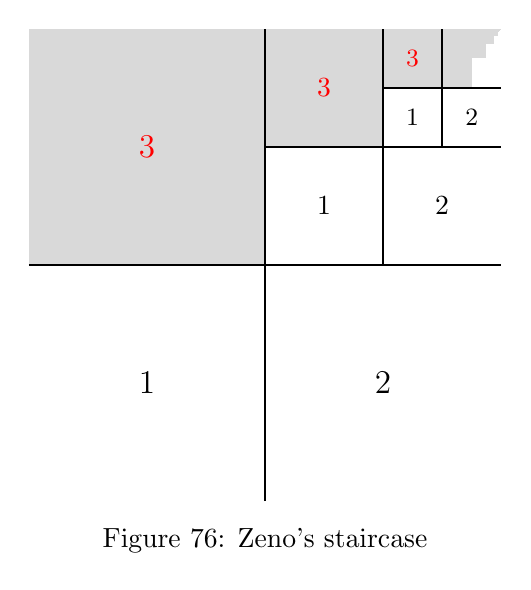
\begin{tikzpicture}
        % Draw the large square (6x6 units)
        \fill[gray!30] (0,0) rectangle (6,6);

        % Draw the staircase starting with the largest rectangle (1/4 area)
        \fill[white] (0,0) rectangle (3,3);  % First step (1/4 of the square)
        \fill[white] (3,0) rectangle (4.5,4.5);  % Second step (1/2 of the remaining area)
        \fill[white] (4.5,0) rectangle (6,5.25);  % Third step (1/2 of remaining)
        \fill[white] (5.625,5.25) rectangle (6,5.625);  % Fourth step
        \fill[white] (5.8125,5.625) rectangle (6,5.8125);  % Fifth step
        \fill[white] (5.90625,5.8125) rectangle (6,5.90625);  % Sixth step
        \fill[white] (5.953125,5.90625) rectangle (6,5.953125);  % Seventh step
        \fill[white] (5.9765625,5.953125) rectangle (6,5.9765625);  % Eighth step
        \fill[white] (5.98828125,5.9765625) rectangle (6,5.98828125);  % Ninth step
        \fill[white] (5.994140625,5.98828125) rectangle (6,5.994140625);  % Tenth step

        % Draw a vertical line through the middle
        \draw[thick] (3,0) -- (3,6);  % Vertical line through the center
        % Draw a horizontal line through the middle
        \draw[thick] (0,3) -- (6,3);  % Horizontal line through the center
        \node at (1.5, 1.5) {\large 1};
        \node at (4.5, 1.5) {\large2};
        \node[red] at (1.5, 4.5) {\large3};
% Draw a vertical line through the middle
        \draw[thick] (4.5,3) -- (4.5,6);  % Vertical line through the center
        % Draw a horizontal line through the middle
        \draw[thick] (3,4.5) -- (6,4.5);  % Horizontal line through the center
        \node at (3 + 6/8, 3 + 6/8) { 1};
        \node at (5.25, 3 + 6/8) { 2};
        \node[red] at (3 + 6/8, 5.25) { 3};
        
        \draw[thick] (4.5 + 6/8,4.5) -- (4.5 + 6/8,6);  % Vertical line through the center
        % Draw a horizontal line through the middle
        \draw[thick] (4.5, 4.5 + 6/8) -- (6, 4.5 + 6/8);  % Vertical line through the center
        \node at (4.5 + 3/8, 4.5 + 3/8) {\small 1};
        \node at (4.5 + 3/8 + 6/8, 4.5 + 3/8) {\small 2};
        \node[red] at (4.5 + 3/8, 4.5 + 3/8 + 6/8) {\small 3};
        % Label the figure
        \node at (3,-0.5) {Figure 76: Zeno's staircase};
    \end{tikzpicture}
    \]
    Thus, we have that the area is $\frac{2}{3}.$\\

    
    Zeno's staircase is constructed as follows: \[Z(x) = \sum_{k=1}^n\frac{1}{2^k}, x\in [\sum_{k=1}^{n-1}\frac{1}{2^k}, \sum_{k=1}^n\frac{1}{2^k}).\] For example, for $n=1,$ we have that $Z(x) = \frac{1}{2}$ for $x\in [0, \frac{1}{2}).$ and $Z(x) = \frac{3}{4}$ for $x\in [\frac{1}{2}, \frac{3}{4}).$ We have that $Z$ is integrable on $[0,1]$ by the Riemann-Lebesgue, since the set of discontinuities is countable, since each one happens every $\frac{2^n -1}{2^n}.$ Thus, we have that 
    \begin{align*}
        \int_0^1 Z(x) &= \int_0^\frac{1}{2}Z(x) + \int_\frac{1}{2}^\frac{3}{4}Z(x) + \int_\frac{3}{4}^{\frac{7}{8}}Z(x) + \dots\\
        &= \lim_{n\to \infty}\sum_{k=1}^n\int_{\sum_{k=1}^{n-1}\frac{1}{2^k}}^{\sum_{k=1}^n\frac{1}{2^k}}\sum_{k=1}^n\frac{1}{2^k}dx\\
        &= \lim_{n\to \infty }\left(\frac{1}{2}\frac{1}{2} + \frac{1}{4}\frac{3}{4} + \frac{1}{8}\frac{7}{8} + \dots + \frac{1}{2^n}\sum_{k=1}^n\frac{1}{2^k}\right)\\
        &= \lim_{n\to \infty} \left(\sum_{k=1}^n\frac{1}{2^k}\frac{2^{k}-1}{2^k}\right)\\
        &= \lim_{n\to \infty}\left(\sum_{k=1}^n\frac{2^k -1}{2^{2k}}\right)\\
        &= \lim_{n\to \infty}\left(\sum_{k=1}^n(\frac{1}{2})^k - \sum_{k=1}^n(\frac{1}{4})^k\right)\\
        &= 2- \frac{4}{3}\\
        &= \frac{2}{3}.
    \end{align*} Where we used the geometric series formula.
    \end{solution}
\item 
\begin{problem}
    What about the Devil’s staircase?
\end{problem}
\begin{solution}
We claim that the devil's staircase satisfies the following for all $c\in [0,1]$
\[H(x)  + H(1-x) = 1.\] 
Let $x\in C,$ then $x$ can be uniquely expressed by 
\[x = 0.\omega_1\omega_2, \dots,\] where $\omega_i$ is $0,$ $1$ or ,$2$  The cantor function will send $x\in C$ to 
\[H(x) = \sum_{i=1}^\infty \frac{\omega_i/2}{2^i}.\] If $x\notin C,$ $H$ has equal values at the endpoints of the discarded gap intervals and so we extend
$H$ to them by letting it be constant on each. Thus, suppose $x\in [0,1],$ then we have that $1 - x=  0.\omega_1'\omega_2', \dots,$ where \[\omega_i' = 2 - \omega_i\] Thus, we have that if $x\in C,$ then $1-x \in C$ (still just expressed in $0$ and $2$) and using the geometric series convergence formula, we have that
\[H(x) + H(1-x) = \sum_{i=1}^\infty \frac{\omega_i/2}{2^i} + \sum_{i=1}^\infty \frac{\omega_i'/2}{2^i} = \sum_{i=1}^\infty \frac{\omega_i/2}{2^i} + \sum_{i=1}^\infty \frac{(2- \omega_i)/2}{2^i} + \sum_{i=1}^\infty \frac{2}{2^{i+1}} = 1.\] We ignore $x\in [0,1]\sm C$ since we just extend the values at the discarded gap intervals, and so we can extend this result to those points.  Thus,
\[\int_0^1H(x) + \int_0^1H(1-x)dx = \int_0^11dx = 1,\] and thus using $u = 1-x$ and $\frac{du}{dx} = -1,$ we have 
\[\int_0^1(H(x) + H(1-x))dx = \int_0^1H(x)dx - \int_1^0H(u)dx = \int_0^1H(x)dx + \int_0^1H(u)dx = 2\int_0^1H(x)dx.\]
Thus, we have that $\int_0^1H(x)dx = \frac{1}{2}.$
\end{solution}
\end{enumerate}
\newpage
\section*{Problem 8}
\begin{enumerate}
    \item 
    \begin{problem}
    Construct a function $f:[-1,1]\to \bbR$ such that 
    \[\lim_{r\to 0}\left(\int_{-1}^{-r}f(x)dx + \int_r^1f(x)dx\right)\] exists but the integral $\int_{-1}^1$ does not exist.    
    \end{problem}
    \begin{solution}
    Consider $f:[-1,1]\to \bbR$ such that 
    \[f(x) = 
    \begin{cases}
        \frac{1}{x}, \qquad x\neq 0\\
        0, \qquad x = 0
    \end{cases}\] We have that \[\lim_{r\to \infty}\left(\int_{-1}^{-r}\frac{1}{x}dx + \int_r^1 \frac{1}{x}dx\right) = 0\] because of symmetry. However, when considering the full interval, $0$ must be included in some subinterval, and thus we would have that "height" of the Riemann rectangle would be infinite, implying that $\int_{-1}^1 f$ does not exist.
    \end{solution}
    \item 
    \begin{problem}
    Do the same for a function $g: \bbR \to \bbR$ such that \[\lim_{R\to \infty}\int_{-R}^Rg(x)dx\] exists but $\int_{-\infty}^\infty g(x)dx$ fails to exist.
    \end{problem}
    \begin{solution}
        Consider $g: \bbR$ to $\bbR$ such that 
        \[g(x) = x^3.\] Because of symmetry and for the same reason as above, we have that the first integral exists and equals $0$:
        \[\lim_{R\to \infty}\int_{-R}^R g(x)dx = \lim_{R\to \infty}\left(\int_{-R}^0g(x)dx + \int_0^Rg(x)dx\right) = 0.\]
        However, we have that \[\left(\int_{-\infty}^0g(x)dx + \int_0^\infty g(x)dx\right) = \infty - \infty,\] which is indeterminate.
    \end{solution}
\end{enumerate}
\newpage


\section*{Problem 9}
\begin{enumerate}
    \item 
\begin{problem}
If $\sum a_n$ converges and $(b_n)$ is monotonic and bounded, prove that $\sum a_nb_n$ converges.
\end{problem}
\begin{solution}
    We claim that if $(c_n)\to 0$ is monotone decreasing, then $\sum a_k c_n$ converges. By Luis' hint during office hours, we have that:
    \begin{align*}
    \sum_{k=1}^{n-1}A_k(c_k - c_{c+1}) &= A_1(c_1 -c_2) + A_2(c_2 - c_3)+ \dots\\
    &= \sum_{k=1}^{n-1}a_kc_k -  A_{n-1}c_{n},
    \end{align*} which can be proved by induction.
    We have that since $A_n$ converges, then it is bounded by some $|A_k|\leq A.$ Thus, we note that since $c_{k} - c_{k+1}\geq 0$ for all $k,$ then
    \begin{align*}
        \left|\sum_{k=m+1}^n a_k c_k\right| &= \left|\sum_{k=1}^{n-1}A_k(c_k - c_{k+1}) + A_{n-1}c_n - (\sum_{k=1}^mA_k(c_{k} - c_{k+1}) + A_mc_{m+1})\right|\\
        &= \left| \sum_{k=m+1}^{n-1}A_k(c_{k} - c_{k+1}) + A_{n-1}c_n + A_mc_{m+1}\right|\\
        &\leq \left| \sum_{k=m+1}^{n-1}A(c_{k} - c_{k+1}) + Ac_n + Ac_{m+1}\right|\\
        &\leq A\left(\sum_{k=m+1}^{n-1}(c_k - c_{k+1}) + c_n + c_{m+1}\right)\\
        &= A \left(2c_{m+1}\right)\\
        &< 2A\frac{\epsilon}{2A}.\\
    \end{align*}
    The last inequality comes from the fact that $c_n \to 0.$ Suppose that $b_n$ is monotone increasing and bounded. Thus, it converges to some $b.$ Let $c_n = b- b_n.$ Then we have that $c_n \to 0$ and $c_n$ is monotonically decreasing. Thus, by the work above, we have that 
    \[\sum_{k=1}^n a_k(b-b_k) = b\sum_{k=1}^na_k - \sum_{k=1}^n a_kb_k\] converges. Since $b\sum_{k=1}^n a_k$ converges, then $\sum_{k=1}^n a_k b_k$ converges. Suppose $b_n$ is monotone decreasing and bounded, then $b_n -b\to 0$ and  $c_n = b_n - b$ is monotone decreasing. Thus, we can use the same strategy as above to show that $\sum a_kb_k$ converges.
\end{solution}
\item 
\begin{problem}
    If the monotonicity condition is dropped, or replaced by the assumption that $\lim_{n\to \infty} b_n = 0,$ find a counter-example to convergence of $\sum a_nb_n.$
\end{problem}
\begin{solution}
    Suppose the monotonicity example is dropped. Then let $b_n = \frac{(-1)^n}{n^{\frac{1}{2}}}$ and let $a_n = b_n.$ We know that $a_n\to 0$ and that $\sum a_n$ converges by alternating series test. We have that $b_n$ is not monotonic and $b_n \to 0$. Thus, we have that 
    \[\sum a_nb_n = \sum \frac{(-1)^n}{n^{\frac{1}{2}}}\frac{(-1)^n}{n^{\frac{1}{2}}} = \sum \frac{1}{n},\] which does not converge.
\end{solution}
\end{enumerate}

\newpage
\section*{Problem 10}
\begin{problem}
    An infinite product is an expression $\prod c_k$ where $c_k>0$. The nth partial
 product is $C_n = c_1\cdots c_n.$ If $C_n$ converges to a limit $C\neq 0$ then the product
 converges to $C$. Write $c_k =1+a_k$. If each $a_k \geq 0$ or each $a_k \leq 0$ prove that $\sum a_k$ converges if and only if $\prod c_k$ converges.
\end{problem}
\begin{solution}
We claim that if $|a_k|\leq 1,$ we have that
        \begin{align}
            1 + \sum_{k=1}^n(a_k) \leq \prod_{k=1}^{n}(1 + a_k)\leq e^{\sum_{k=1}^n(a_k)}
        \end{align}
        To see the first inequality, consider that we can expand the right side:
        \begin{align*}
        \prod_{k=1}^n (1 +a_k) &= (1 + a_1)(1+a_2)(1 + a_3) \cdot \dots \cdot (1 + a_n)\\
        &= (1 + a_1 + a_2+a_1a_2)(1 + a_3) \cdot \dots  \cdot (1 + a_n)\\
        &= 1 + a_1 + a_2 + a_1a_2 + a_3 + a_1a_4 + a_2a_3 +a_1a_2a_3\cdot \dots \cdot (1+a_n)\\
        &= 1 + \sum a_n + K,
        \end{align*}
        where $K$ is some constant. That is, the product of the sum contains the sum in it. To see the second inequality, we need to show that 
        \begin{align}
                    \ln(1 + a_k)\leq a_k.
        \end{align}
        To see this, consider that this is equivalent to showing that 
        \[1 + a_k \leq e^{a_k} \iff 0 \leq e^x - (1 + x) = f(x)\] for $|x|< 1$ (since $c_k > 0.$) Consider that by taking derivatives, we have that
        \[f'(x) = e^x - 1, \qquad f''(x) = e^x.\] Thus, $f(x)$ has a critical point at $x=0,$ and $f(x)$ is concave up, so $x=0$ is the local minimum for $-1<x<1.$ Thus, $0\leq e^x - (1 + x)$ for all $|x|<1.$ Thus, we have (4), implying that 
        \[\sum_{k=1}^n\ln(1 + a_k)\leq \sum_{k=1}^na_k.\] Thus, using logarithm rules, we have that 
        \[\ln\left(\prod_{k=1}^n (1 + a_k)\right)\leq \sum_{k=1}^na_k\iff \prod_{k=1}^n(1 + a_k) \leq e^{\sum_{k=1}^na_k}.\]
    \begin{itemize}
        \item 
        $(\implies):$ Suppose $\sum a_k$ converges, then since $c_k = 1 + a_k >0,$ we must have that $|a_k|<1$ for large $k.$ By (3), we have that for large $m,$
        \[0\leq \prod_{k=m+1}^n c_k \leq e^{\sum_{k=m+1}^n a_k},\] and thus since $\ln$ is continuous and monotonic, we have that
        \[\ln\left(\prod_{k=1}^n c_k\right) \leq {\sum_{k=1}^n a_k},\] and thus \[\sum\left(\ln(1 + a_k)\right) \leq e^{\sum_{k=m+1}^n a_k}.\] Thus, if $a_k \geq 0$ for all $k,$ then $|\ln(1 + a_k)| = \ln(1 + a_k)\leq a_k,$ and thus the series converges by the comparison test. If $a_k\leq 0$ for all $k,$ then $\ln(1+a_k)$ since $a_k \to 0,$ we have that $\ln(1 + a_k)$ is increasing. Thus, if $\sum_{k= m+1}^n\ln(1 + a_k)$ is an increasing sequence of partial sums that is bounded above, and thus converges. Thus, since $\ln$ is continuous, we have that 
        \[\lim_{n\to \infty}\ln\left(\prod_{k=m+1}^n c_k\right) = \ln\left(\lim_{n\to \infty}\prod_{k=m+1}^n c_k\right),\] and so we must have that $\prod c_k$ converges. 
        \item ($\impliedby$): Suppose $\prod c_k$ converges. Since $c_k = 1 + a_k>0,$ then we must have for large $k,$ $|a_k|<1.$ Thus, by (3), we have that for large $m,$
        \[1 + \sum_{k=m+1}^n a_k \leq \prod_{k=m+1}^n c_k \leq e^{\sum a_k}.\] Thus, we have that if $a_k\geq 0$ for all $k,$ then the tail of $\sum a_k$ is increasing and bounded above and thus converges. If $-1<a_k \leq 0$ for all $k,$ then $\sum_{k=1}^n a_k = A_n$ is decreasing, and thus $e^{A_n}$ is decreasing and positive, and thus the tail of $e^{A_n}$ is decreasing and bounded below by our product, and thus converges.
    \end{itemize}
\end{solution}
\begin{reflection}
    An alternative method would be to use $L'hopital.$ \[\lim_{k \to \infty}\frac{\ln(1 + a_k)}{a_k} = \lim_{x\to 0}\frac{\ln(1+x)}{x} = \lim_{x\to 0}\frac{1}{1+x} = 1,\] and thus we have that for large enough $k,$ $\ln(1+a_k) = a_k.$ Thus, for large $n,m:$
        \[\sum_{k=m+1}^n\ln(1+a_k) = \sum_{k=m+1}^n a_k + 
        \epsilon,\]
\end{reflection}
\end{document}